\documentclass[tikz,border=10pt]{standalone}
\usepackage{tikz}
\usepackage{verbatim}
\begin{document}

\tikzset{every picture/.style={line width=0.75pt}} %set default line width to 0.75pt

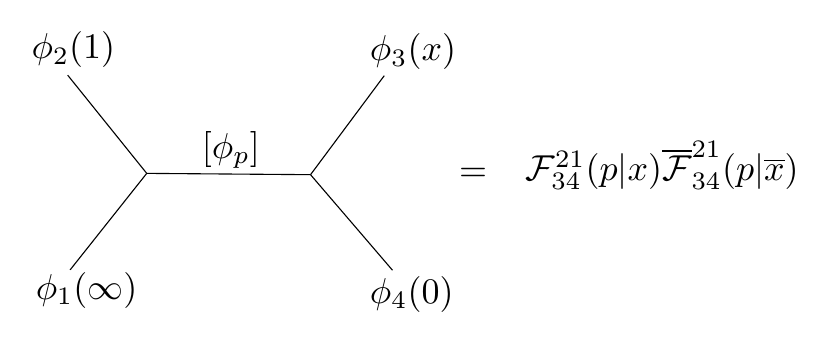
\begin{tikzpicture}[x=0.75pt,y=0.75pt,yscale=-1,xscale=1]
%uncomment if require: \path (0,300); %set diagram left start at 0, and has height of 300

%Straight Lines [id:da1631152617286873]
\draw    (170,72) -- (208.09,119.33) ;
%Straight Lines [id:da7190082045963415]
\draw    (208.09,119.33) -- (171.18,165.83) ;
%Straight Lines [id:da2417815563038921]
\draw    (208.09,119.33) -- (287.02,119.96) ;
%Straight Lines [id:da8962007926432798]
\draw    (326.5,166) -- (287.02,119.96) ;
%Straight Lines [id:da8114709389430173]
\draw    (287.02,119.96) -- (322.53,72.26) ;

% Text Node
\draw (153,165.4) node [anchor=north west][inner sep=0.75pt,scale=1.3]    {$\phi _{1}( \infty )$};
% Text Node
\draw (151,49.4) node [anchor=north west][inner sep=0.75pt,scale=1.3]    {$\phi _{2}( 1)$};
% Text Node
\draw (314,50.4) node [anchor=north west][inner sep=0.75pt,scale=1.3]    {$\phi _{3}( x)$};
% Text Node
\draw (314,167.4) node [anchor=north west][inner sep=0.75pt,scale=1.3]    {$\phi _{4}( 0)$};
% Text Node
\draw (233,97.4) node [anchor=north west][inner sep=0.75pt,scale=1.3]    {$[ \phi _{p}]$};
% Text Node
\draw (357,115.4) node [anchor=north west][inner sep=0.75pt,scale=1.3]    {$=$};
% Text Node
\draw (389,102.4) node [anchor=north west][inner sep=0.75pt,scale=1.3]    {$\mathcal{F}_{34}^{21}( p|x)\overline{\mathcal{F}}_{34}^{21}( p|\overline{x})$};


\end{tikzpicture}
\end{document}
